\documentclass{article}
\usepackage{tikz}
\usepackage{xcolor}

\begin{document}

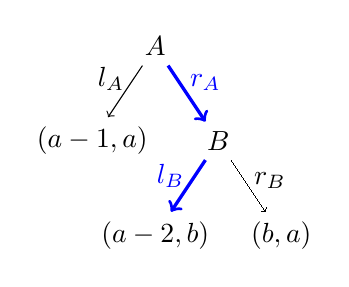
\begin{tikzpicture}
    [
        level 1/.style = {->, sibling distance = 1.6cm},
        level 2/.style = {->, sibling distance = 1.6cm}
    ]

    \node {$A$}
        child {
        node [yshift = 0.3cm] {$(a-1,a)$}
        edge from parent node [left, pos=0.25] {$l_A$}
        }
        child {
            node [yshift = 0.3cm]  {$B$}
            child {
                node [yshift = 0.3cm] {$(a-2, b)$}
                edge from parent [blue, very thick] node [left, pos=0.3] {$l_B$}
                }
            child {
                node [yshift = 0.3cm] {$(b, a)$}
                edge from parent [black, line width = 0pt] node [right, pos=0.4] {$r_B$}
                }
            edge from parent [blue, very thick] node [right, pos=0.3] {$r_A$}
            };
    \end{tikzpicture}

\end{document}